\documentclass[11pt,a4paper]{article}

% ============================================================
% PACKAGES
% ============================================================
\usepackage[a4paper,top=0.75in,bottom=0.75in,left=0.8in,right=0.8in]{geometry}
\usepackage[T1]{fontenc}
\usepackage[utf8]{inputenc}
\usepackage{mathptmx}
\usepackage{microtype}
\usepackage{parskip}
\usepackage{enumitem}
\usepackage{booktabs}
\usepackage{tabularx}
\usepackage{array}
\usepackage{graphicx}
\usepackage{caption}
\usepackage{titlesec}
\usepackage{xcolor}
\usepackage{tikz}
\usepackage[hidelinks]{hyperref}
\usepackage{xurl}
\usetikzlibrary{shapes.geometric, arrows.meta, positioning, fit, backgrounds, calc}

% Professional section spacing
\titlespacing*{\section}{0pt}{11pt}{5pt}
\titlespacing*{\subsection}{0pt}{8pt}{3pt}
\titleformat{\section}{\normalfont\large\bfseries}{\thesection.}{0.5em}{}
\titleformat{\subsection}{\normalfont\normalsize\bfseries}{\thesubsection}{0.5em}{}

\setlist[itemize]{leftmargin=1.4em,topsep=3pt,itemsep=3pt,parsep=0pt}
\setlist[enumerate]{leftmargin=1.6em,topsep=3pt,itemsep=3pt,parsep=0pt}

% Color palette for architecture diagram
\definecolor{boxblue}{RGB}{41,128,185}
\definecolor{boxgreen}{RGB}{39,174,96}
\definecolor{boxorange}{RGB}{230,126,34}
\definecolor{boxpurple}{RGB}{142,68,173}
\definecolor{boxgray}{RGB}{120,120,120}
\definecolor{lightblue}{RGB}{213,232,255}
\definecolor{lightgreen}{RGB}{213,245,218}
\definecolor{lightorange}{RGB}{255,229,204}
\definecolor{lightpurple}{RGB}{235,218,245}
\definecolor{lightgray}{RGB}{240,240,240}

\setlength{\parskip}{5pt}
\setlength{\parindent}{0pt}
\linespread{1.09}\selectfont

% ============================================================
% TITLE BLOCK
% ============================================================
\begin{document}

\begin{center}
{\Large\bfseries Smart Workout: A RAG-Assisted Decision Support and \\[2pt]
Business Intelligence System for Personalized Weight Training}\\[6pt]
{\normalsize Project Proposal\,---\,Business Intelligence and Analytics}
\end{center}

\begin{center}
\small
\begin{tabular}{lll}
\textbf{Aye Khin Khin Hpone} (Yolanda Lim) & \textbf{Waranon Neamtuptim} (Non) & \textbf{Jirapat Datephanyawat} (Earth) \\
ID: st125970 & ID: st125934 & ID: st125843 \\
\end{tabular}
\end{center}

% ============================================================
% 1. BACKGROUND
% ============================================================
\section{Background}
Weight training is widely practiced for strength and fitness, yet many gym users struggle to plan effectively: they are uncertain which exercises suit a given body part, how to adapt to available equipment, how to structure a weekly timetable, and whether their physical condition supports a particular plan. Most decisions come from generic online routines that ignore personal factors --- age, sleep, BMI, physiological indicators, equipment, schedule --- producing a mismatch between plan and readiness. This project proposes \textbf{Smart Workout}, a combined Decision Support System (DSS) and Business Intelligence System (BIS) (Power, 2002; Chaudhuri et al., 2011) that unifies multi-source real-world data, a Retrieval-Augmented Generation (RAG) knowledge layer, and supervised ML models behind an interactive web dashboard, transforming raw input into descriptive insight, predictive outcome estimates, and prescriptive training plans while preserving human oversight. Intended end users are gym users seeking personalized training guidance; fitness coaches form a secondary audience using the dashboard for decision-support reference.

% ============================================================
% 2. OBJECTIVES
% ============================================================
\section{Objectives}
The project will deliver a working DSS/BIS prototype that fulfils the following objectives, explicitly covering the descriptive, predictive, and prescriptive analytics layers required of a BI system:
\begin{itemize}
  \item \textbf{Data collection \& preparation:} clean and standardize multi-source public datasets (gym membership and check-in records, exercise catalogue, gym-member workout tracking, sleep \& lifestyle, daily nutrition; details in \S4) plus structured user input.
  \item \textbf{Descriptive analytics:} segment users into lifestyle profiles via clustering on the sleep dataset, and present multi-dataset exploratory insights (calorie-burn patterns, exercise coverage, nutrition macro mix) on the dashboard.
  \item \textbf{Predictive analytics:} train and compare multiple candidate models per task via cross-validation: (a) \emph{calorie-burn-rate} regression (kcal\,/\,hr); (b) \emph{Workout Intensity} 3-class classification (Low/Mid/High). A rule-derived \emph{Training Readiness} band (computed from user input; rules drawn from the Sleep Health dataset) guides the plan generator (see \S5).
  \item \textbf{Prescriptive analytics:} generate a daily/weekly training plan via a rule-based engine conditioned on the predicted intensity, readiness, target body part, and available equipment; the predicted calorie-burn rate is displayed alongside the plan.
  \item \textbf{RAG knowledge retrieval \& AI chat assistant:} retrieve exercise instructions, equipment-substitution rules, and timetable guidance via a pop-up chat widget (RAG retrieval is core; LLM chat is a planned extension).
  \item \textbf{BI dashboard:} React-based dashboard (with embedded Tableau views) presenting a relational gym membership view, multi-dataset descriptive analytics, personalized predictions, prescribed plan, RAG-sourced explanation, and embedded chat.
\end{itemize}

% ============================================================
% 3. SYSTEM DESCRIPTION & ARCHITECTURE
% ============================================================
\section{Description of the Proposed DSS/BIS}
Smart Workout will be developed as a React + FastAPI web application integrating multi-source data, trained and evaluated models (selected after comparing multiple candidates per task via cross-validation; see \S5), a vector store-based RAG knowledge layer (Lewis et al., 2020), a rule-based plan generator, and an embedded chat assistant powered by RAG retrieval, with optional LLM enhancement. The selected regressor and classifier run on every user request and provide input to the prescriptive plan generator; the chat reuses the same RAG pipeline so its answers are grounded in the indexed corpus rather than parametric memory. The system architecture and end-to-end workflow are illustrated in Figure~\ref{fig:arch}. The technology stack comprises React with embedded Tableau dashboards (frontend), FastAPI (backend), pandas, scikit-learn, and XGBoost (analytics), a vector store with sentence embeddings (RAG), and a general-purpose LLM such as OpenAI GPT or Grok for chat and explanation.

\begin{figure}[h]
\centering
\resizebox{0.98\linewidth}{!}{
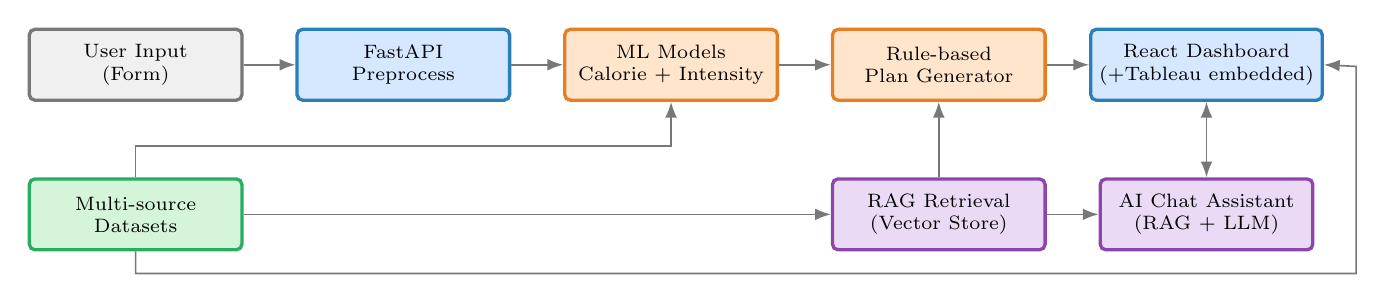
\begin{tikzpicture}[
  every node/.style={font=\scriptsize},
  box/.style={rectangle, rounded corners=2pt, draw, very thick, minimum height=9mm, minimum width=27mm, align=center, inner sep=3pt},
  user/.style={box, fill=lightgray, draw=boxgray},
  app/.style={box, fill=lightblue, draw=boxblue},
  data/.style={box, fill=lightgreen, draw=boxgreen},
  ml/.style={box, fill=lightorange, draw=boxorange},
  rag/.style={box, fill=lightpurple, draw=boxpurple},
  arr/.style={-{Latex[length=2mm]}, semithick, draw=boxgray},
  biarr/.style={{Latex[length=2mm]}-{Latex[length=2mm]}, semithick, draw=boxgray}
]
% Row 1 (y=1.9): runtime pipeline (5 boxes, evenly spaced)
\node[user] (input) at (0,    1.9) {User Input\\(Form)};
\node[app]  (api)   at (3.4,  1.9) {FastAPI\\Preprocess};
\node[ml]   (ml)    at (6.8,  1.9) {ML Models\\Calorie + Intensity};
\node[ml]   (plan)  at (10.2, 1.9) {Rule-based\\Plan Generator};
\node[app]  (dash)  at (13.6, 1.9) {React Dashboard\\(+Tableau embedded)};
% Row 2 (y=0): supporting + interactive layer
%   RAG aligned vertically with Plan; Chat aligned vertically with Dashboard
\node[data] (data)  at (0,    0)   {Multi-source\\Datasets};
\node[rag]  (rag)   at (10.2, 0)   {RAG Retrieval\\(Vector Store)};
\node[rag]  (chat)  at (13.6, 0)   {AI Chat Assistant\\(RAG + LLM)};

% top pipeline (4 horizontal arrows)
\draw[arr] (input) -- (api);
\draw[arr] (api)   -- (ml);
\draw[arr] (ml)    -- (plan);
\draw[arr] (plan)  -- (dash);

% Data -> RAG (long horizontal through empty row 2, no boxes in the way)
\draw[arr] (data) -- (rag);

% Data -> ML (training-time feed; clean elbow up-then-right, well above row 2 boxes and below row 1 boxes)
\draw[arr] (data.north) -- ++(0,0.4) -| (ml.south);

% RAG -> Plan (clean vertical, aligned columns)
\draw[arr] (rag) -- (plan);

% RAG -> Chat (short horizontal)
\draw[arr] (rag) -- (chat);

% Dashboard <-> Chat (bidirectional vertical, aligned columns)
\draw[biarr] (dash) -- (chat);

% Data -> Dashboard (Tableau descriptive feed; routes below and right of all boxes)
\draw[arr] (data.south) -- ++(0,-0.28) -- ++(15.5,0) -- ++(0,2.63) -- (dash.east);
\end{tikzpicture}
}
\caption{Smart Workout system architecture and workflow.}
\label{fig:arch}
\end{figure}

\textbf{End-to-end workflow (Figure~\ref{fig:arch}).} User input $\rightarrow$ FastAPI preprocessing $\rightarrow$ ML models predict calorie-burn rate and intensity $\rightarrow$ RAG retrieves instructions and rule snippets $\rightarrow$ rule-based generator assembles the plan with optional LLM explanation $\rightarrow$ dashboard renders plan, predictions, and chat.

% ============================================================
% 4. DATA SOURCES
% ============================================================
\section{Data Sources}
Five publicly available datasets are used across the system, each serving a distinct role. The gym membership dataset provides a relational star schema (users, check-ins, subscription plans, gym locations linked by shared keys) as the primary Tableau descriptive source; the remaining datasets support ML training, RAG retrieval, lifestyle clustering, and nutrition context.

\vspace{-2pt}
\begin{center}
\small
\renewcommand{\arraystretch}{1.1}
\begin{tabularx}{\linewidth}{l r X}
\toprule
\textbf{Dataset} & \textbf{Records} & \textbf{Role in the system} \\
\midrule
\href{https://www.kaggle.com/datasets/amoghabhinavms/gym-database-management-system}{Gym Database Management System} (Amoghabhinavms, n.d.) & 305{,}013 & Four linked tables (users, check-ins, subscription plans, gym locations). Primary Tableau descriptive source; gym type and facilities inform location-level plan constraints. \\
\href{https://exercisedb.dev/}{ExerciseDB (raw flat)} (ExerciseDB, n.d.) & 1{,}500 & Exercise catalogue (body parts, equipment, target muscles, instructions). Powers the exercise recommender and RAG. \\
\href{https://www.kaggle.com/datasets/valakhorasani/gym-members-exercise-dataset}{Gym Members Exercise Tracking} (Khorasani, 2024) & 973 & Workout sessions with calories, BPM, duration, workout type, BMI, experience. Primary ML training data. \\
\href{https://www.kaggle.com/datasets/uom190346a/sleep-health-and-lifestyle-dataset}{Sleep Health \& Lifestyle} (Tharmalingam, 2023) & 374 & Lifestyle cluster basis; rule source for \emph{Training Readiness} computed from user input. \\
\href{https://www.kaggle.com/datasets/adilshamim8/daily-food-and-nutrition-dataset}{Daily Food Nutrition} (Shamim, 2025) & 651 & Macro/calorie context on the dashboard; nutrition-aware snippets embedded in RAG. \\
\bottomrule
\end{tabularx}
\end{center}

% ============================================================
% 5. METHODS
% ============================================================
\section{Methods: Descriptive, Predictive, Prescriptive}
\textbf{Descriptive:} Clustering on the Sleep \& Lifestyle dataset identifies several user archetypes. The Tableau descriptive layer presents a relational gym membership view --- member activity patterns, subscription trends, and usage analytics --- powered by the Gym Database Management System star schema, alongside cross-dataset exploratory views (calorie-burn patterns, exercise coverage, nutrition macro mix).

\textbf{Predictive:} For each predictive task, multiple candidate models well-suited to a moderately-sized tabular problem are trained and compared, with the best selected via cross-validation. The candidate set spans an interpretable linear baseline, a robust bagged-tree ensemble, and a state-of-the-art boosted-tree model:
\begin{itemize}
  \item \textbf{Calorie-burn-rate regression} (kcal\,/\,hr; session duration excluded so the model learns physiology): \emph{Ridge Regression}, \emph{Random Forest Regressor}, \emph{XGBoost Regressor} (Chen \& Guestrin, 2016). Metrics: RMSE, MAE, $R^2$.
  \item \textbf{Workout-intensity classification} (3-class Low/Mid/High, derived from BPM indicators; label-derived features excluded from inputs): \emph{Multinomial Logistic Regression}, \emph{Random Forest Classifier}, \emph{XGBoost Classifier}. Metrics: accuracy, macro-F1, confusion matrix.
\end{itemize}
SHAP (Lundberg \& Lee, 2017) is applied to the selected models for feature-importance attribution shown in the dashboard.

\textbf{Prescriptive:} A rule-based generator combines predicted intensity, readiness, target body part, and the exercise recommender's filtered pool into a structured plan (split, exercises, sets, reps, rest). Intensity modulates volume and load (High $\rightarrow$ higher volume, Low $\rightarrow$ reduced load). Gym type and facilities sourced from the gym locations dimension provide location-level context for plan constraints. A vector store (indexing ExerciseDB exercise instructions, nutrition-aware workout snippets from the Daily Food Nutrition dataset, and a curated rule corpus of training guidelines and equipment substitutions, embedded using sentence embeddings) supplies rationale, substitutions, and nutrition-aware guidance to both the plan generator and chat; LLM-powered chat is a planned extension; any compatible AI model (\emph{e.g.}\ OpenAI GPT, Grok) can be integrated when available.

% ============================================================
% 6. EXPECTED OUTPUTS
% ============================================================
\section{Expected Outputs}
A working React + FastAPI prototype with a vector store and trained and evaluated models; a personalized training plan (structured format and dashboard view) including split, exercises, sets/reps, intensity band, predicted calorie-burn rate, and equipment substitutions; predictive insights with class probabilities and SHAP feature attribution; and a multi-view BI dashboard (gym membership, lifestyle profiles, descriptive exploration, prediction + plan, RAG explanation) with an embedded RAG-grounded chat assistant.

% ============================================================
% 7. CONCLUSION (merged: scope, limitations, conclusion)
% ============================================================
\section{Conclusion}
Smart Workout delivers a working DSS/BIS prototype combining multi-source real-world data, supervised ML, a relational Tableau descriptive layer, and a RAG-grounded prescriptive engine. It is a decision-support tool, not a clinical replacement; outputs include class probabilities, cross-validated metrics, and transparent limitations. Core deliverables are the descriptive view, plan generator, retrieval-only RAG, and SHAP attribution; LLM-powered chat is a planned extension.

% ============================================================
% REFERENCES (APA 7th)
% ============================================================
\section*{References}
\vspace{2pt}
\footnotesize
\setlength{\parskip}{2pt}
\begin{list}{}{\setlength{\leftmargin}{1.5em}\setlength{\itemindent}{-1.5em}\setlength{\itemsep}{2pt}\setlength{\parsep}{0pt}\setlength{\topsep}{0pt}}
\item Amoghabhinavms. (n.d.). \emph{Gym database management system} [Data set]. Kaggle. \url{https://www.kaggle.com/datasets/amoghabhinavms/gym-database-management-system}
\item Chaudhuri, S., Dayal, U., \& Narasayya, V. (2011). An overview of business intelligence technology. \emph{Communications of the ACM, 54}(8), 88--98. \url{https://doi.org/10.1145/1978542.1978562}
\item Chen, T., \& Guestrin, C. (2016). XGBoost: A scalable tree boosting system. In \emph{Proceedings of the 22nd ACM SIGKDD International Conference on Knowledge Discovery and Data Mining} (pp. 785--794). ACM. \url{https://doi.org/10.1145/2939672.2939785}
\item ExerciseDB. (n.d.). \emph{ExerciseDB: Free exercise database}. \url{https://exercisedb.dev/}
\item Khorasani, V. (2024). \emph{Gym members exercise dataset} [Data set]. Kaggle. \url{https://www.kaggle.com/datasets/valakhorasani/gym-members-exercise-dataset}
\item Lewis, P., Perez, E., Piktus, A., Petroni, F., Karpukhin, V., Goyal, N., K\"uttler, H., Lewis, M., Yih, W., Rockt\"aschel, T., Riedel, S., \& Kiela, D. (2020). Retrieval-augmented generation for knowledge-intensive NLP tasks. \emph{Advances in Neural Information Processing Systems, 33}, 9459--9474. \url{https://arxiv.org/abs/2005.11401}
\item Lundberg, S. M., \& Lee, S.-I. (2017). A unified approach to interpreting model predictions. \emph{Advances in Neural Information Processing Systems, 30}, 4765--4774.
\item Power, D. J. (2002). \emph{Decision support systems: Concepts and resources for managers}. Quorum Books.
\item Shamim, A. (2025). \emph{Daily food and nutrition dataset} [Data set]. Kaggle. \url{https://www.kaggle.com/datasets/adilshamim8/daily-food-and-nutrition-dataset}
\item Tharmalingam, L. (2023). \emph{Sleep health and lifestyle dataset} [Data set]. Kaggle. \url{https://www.kaggle.com/datasets/uom190346a/sleep-health-and-lifestyle-dataset}
\end{list}

\end{document}
